\begin{figure}
\begin{center}
\begin{minipage}[t]{0.5\linewidth}

% \hspace*{\fill}%
\begin{minipage}[t]{\linewidth}
\centering
\vspace{0pt} % for alignment
\begin{minipage}{\textwidth}
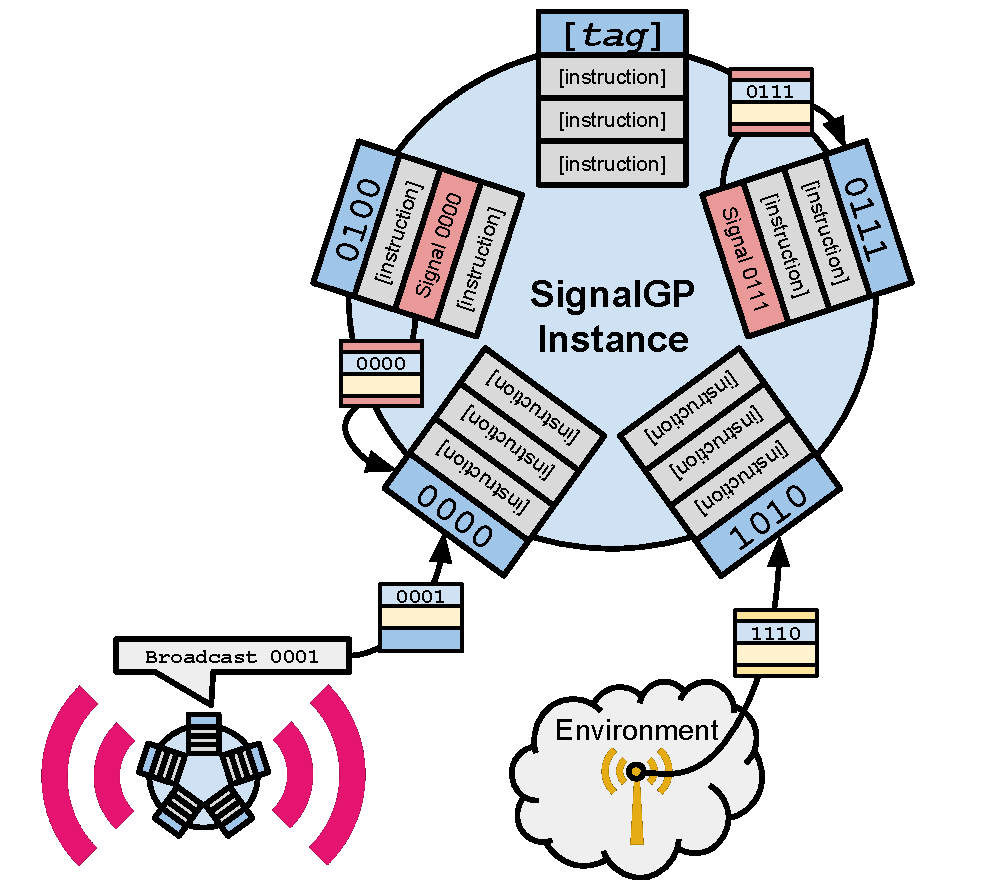
\includegraphics[width=\linewidth]{img/signalgp-cartoon}
{\textbf{(A)}
A cartoon overview of a single SignalGP instance.
SignalGP program modules execute pseudo-concurrently in response to tagged signals, which can originate internally, from the environment, or from other agents.
}
% \label{fig:signalgp-cartoon}
\end{minipage}
\end{minipage}%
% \hspace*{\fill}

% \hspace*{\fill}%
% \begin{minipage}[t]{\linewidth}
% \centering
% \vspace{0pt} % for alignment
% \begin{minipage}{\textwidth}
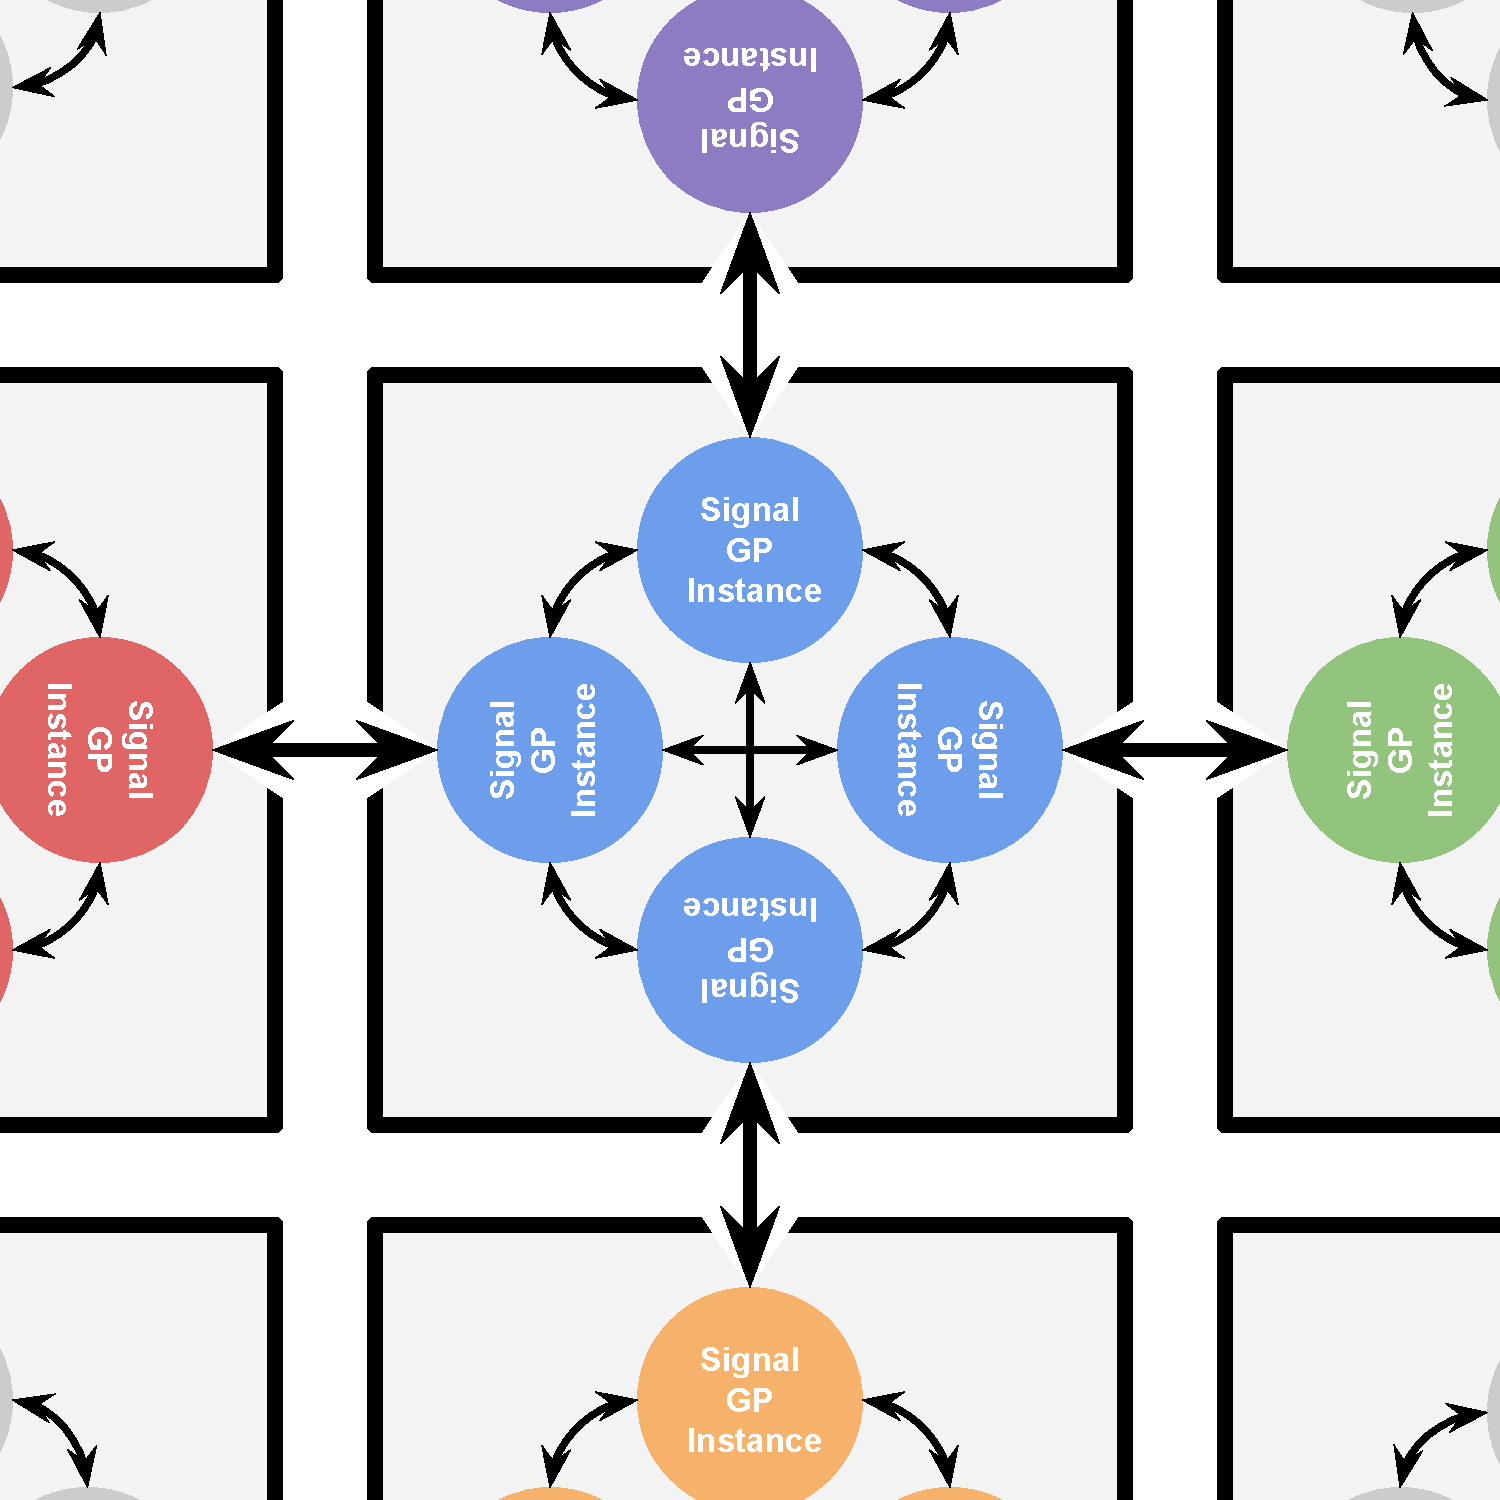
\includegraphics[width=0.8\linewidth]{img/dishtinygp-cartoon}\\
{\textbf{(B)}
A cartoon overview of how individual SignalGP instances are organized into DISHTINY cells.
% Each cell contains four independent SignalGP instances.
% The same genetic program is mirrored across all four SignalGP instances, but each instance executes independently.
Within each DISHTINY cell, each of four independent instances senses environmental state, receives intercellular messages, and determines cell behavior with respect to a single cardinal direction.
All four instances sense non-directional environmental cues and non-directional actions may be taken by any instance.
Instances within a cell communicate via intracellular messaging.
}
% \label{fig:dishtinygp-cartoon}
% \end{minipage}
% \end{minipage}%
% \hspace*{\fill}
\end{minipage}

\caption{
Schematic illustrations of how individual SignalGP instances function and how individual SignalGP instances are organized into DISHTINY cells.
Subfigure \textbf{(A)} provided courtesy Alexander Lalejini.
}
\label{fig:signalgp-dishtinygp}
\end{center}
\end{figure}
